\newcount\draft\draft=1 % set to 0 for submission or publication
\documentclass[sigplan,review,anonymous]{acmart}
\setcopyright{none}
%
\usepackage{tikz}
\usepackage[norelsize]{algorithm2e}
\usepackage{xxx}
\usepackage{fncylab}
\usepackage{subcaption}
%
\usepackage{graphicx}
% Used for displaying a sample figure. If possible, figure files should
% be included in EPS format.
%
% If you use the hyperref package, please uncomment the following line
% to display URLs in blue roman font according to Springer's eBook style:
% \renewcommand\UrlFont{\color{blue}\rmfamily}
\AtBeginDocument{%
  \providecommand\BibTeX{{%
    \normalfont B\kern-0.5em{\scshape i\kern-0.25em b}\kern-0.8em\TeX}}}

\labelformat{algocf}{algorithm\,(#1)}

\begin{document}
\settopmatter{printacmref=false}
\title{Online Verification of Commutativity}
%
%\titlerunning{Abbreviated paper title}
% If the paper title is too long for the running head, you can set
% an abbreviated paper title here
%
\author{First Author}
\email{email}
\author{Second Author}
\authornotemark[1]
\email{email 2}
\affiliation{%
  \institution{Cornell University}
  \streetaddress{address}
  \city{Ithaca}
  \state{New York}
  \postcode{14850}
}

\author{Third Author}
\email{email 3}

\begin{abstract}
Systems of transformations arise in many programming systems, such as in type graphs of implicit type conversion functions.
It is important to ensure that these diagrams commute: that any composing path of transformations from the same source to the same destination yields the same result.
However, a straightforward approach to verifying commutativity must contend with cycles, and even so it runs in factorial time.
While previous work has shown how to verify commutativity in the special case of acyclic diagrams in $O(|V|^4|E|^2)$ time,
% I think this is clear enough (at least for the abstract). --AS
% where V is the set of vertices in the diagram, and E, the set of edges.
but this is a \emph{batch} algorithm: the entire diagram must be known ahead of time.
We present an \emph{online} algorithm that efficiently verifies that a commutative diagram remains commutative when adding a new edge.
The new incremental algorithm runs in $O(|V|^2(|E| + |V|))$ time.
For the case when checking the equality of paths is expensive, we also present an optimization that runs in $O(|V|^4)$ time but reduces to the minimum possible number of equality checks.
We implement the algorithms and compare them to batch baselines, and we demonstrate their practical application in the compiler of a domain-specific language for geometry types.
To study the algorithms' scalability to large diagrams, we apply them to discover discrepancies in currency conversion graphs.
\end{abstract}

\maketitle

\section{Introduction}
Many systems can be understood as diagrams: graphs where nodes represent domains, and edges, directed transformation functions between nodes.
In programming, for example, type systems with coercions can be drawn as a graph with type nodes and coercion edges, as demonstrated in figure ~\ref{fig:typeExample}.
A desirable trait of such a type system and many other similar systems is that traversing the graph from a given start and end node results in the same value independent of path chosen.
A diagram with this property is said to \textit{commute}.
With our type coercion example, it could be problematic if casting to a supposedly equivalent type as an intermediate step resulted in a different answer than a direct cast.

\begin{figure}[]
    \centering
    \begin{subfigure}{.4\textwidth}
        \begin{verbatim}
            var a : meters = 1;
            var b : miles = (miles) a;
            var c : feet = (feet) a;
            define wugs:
                1 miles = 10 wugs;
                1 foot = 10000 wugs;
            var d : wugs = (wugs) a;
        \end{verbatim}
        \caption{A sample program with user defined type conversion.}
    \end{subfigure}

    \begin{subfigure}{.4\textwidth}
        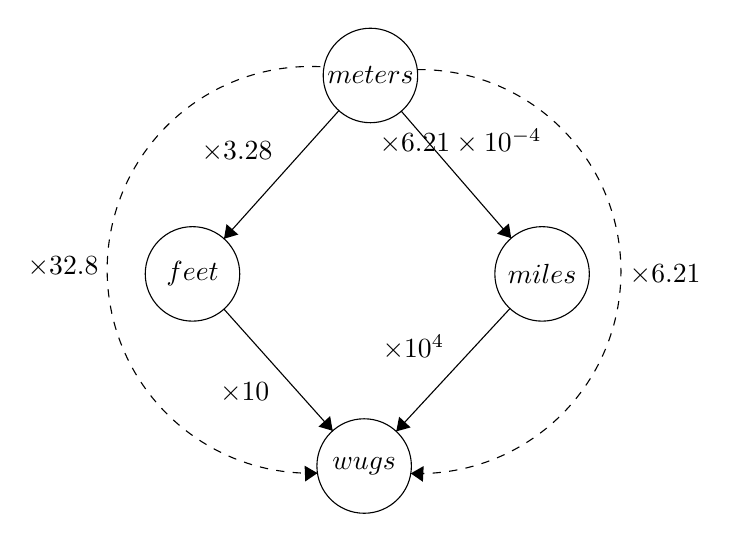
\begin{tikzpicture}[scale=0.2]
            \tikzstyle{every node}+=[inner sep=0pt]
            \draw [black] (32.8,-8.8) circle (3);
            \draw (32.8,-8.8) node {$meters$};
            \draw [black] (21.5,-21.4) circle (3);
            \draw (21.5,-21.4) node {$feet$};
            \draw [black] (43.7,-21.4) circle (3);
            \draw (43.7,-21.4) node {$miles$};
            \draw [black] (32.4,-33.6) circle (3);
            \draw (32.4,-33.6) node {$wugs$};
            \draw [black] (30.8,-11.03) -- (23.5,-19.17);
            \fill [black] (23.5,-19.17) -- (24.41,-18.9) -- (23.66,-18.24);
            \draw (26.61,-13.64) node [left] {$\times 3.28$};
            \draw [black] (34.76,-11.07) -- (41.74,-19.13);
            \fill [black] (41.74,-19.13) -- (41.59,-18.2) -- (40.84,-18.85);
            \draw (43.7,-13) node [left] {$\times 6.21 \times 10^{-4}$};
            \draw [black] (23.5,-23.64) -- (30.4,-31.36);
            \fill [black] (30.4,-31.36) -- (30.24,-30.43) -- (29.5,-31.1);
            \draw (26.41,-28.96) node [left] {$\times 10$};
            \draw [black] (41.66,-23.6) -- (34.44,-31.4);
            \fill [black] (34.44,-31.4) -- (35.35,-31.15) -- (34.62,-30.47);
            \draw (37.52,-26.04) node [left] {$\times 10^4$};
            \draw [dashed] (29.441,-34.049) arc (-88.02206:-273.82603:12.915);
            \fill [black] (29.44,-34.05) -- (28.62,-33.58) -- (28.66,-34.58);
            \draw (15.56,-20.93) node [left] {$\times 32.8$};
            \draw [dashed] (35.77,-8.425) arc (90.49177:-92.33986:12.828);
            \fill [black] (35.36,-34.07) -- (36.13,-34.6) -- (36.18,-33.6);
            \draw (49.23,-21.46) node [right] {$\times 6.21$};
            \end{tikzpicture}
        \caption{Diagram for the type conversions in the program}
    \end{subfigure}

    \caption{In this sample program, the user implicitly defines two ways to cast variable a from meters to the new unit wugs.
    The definitions are different, and a compiler performing implicit conversion would not know which to choose.}
    \label{fig:typeExample}
\end{figure}

Given the utility of system diagram commutativity, it would be useful to check that the property holds for real systems.
Since diagrams may change over time, and verifying the entire system from scratch may be computationally expensive, it would be additionally convenient if new edges could be checked online as they are added.
In figure ~\ref{fig:typeExample}, for example, an interpreter that caught the first instance of a user making a bad definition would need to build and verify the conversion graph at run time.

Naively checking if all path pairs that begin and end at the same node in a given diagram commute could require a number of function equality checks that grow as factorial in the number of nodes, since a path consists of an ordering of nodes.
Further, the presence of cycles implies a potentially infinite number of paths. 
Previous work ~\cite{commutative} has identified an $O(|E|^2|V|^4)$ algorithm to verify that a complete acyclic diagram commutes; however, it addresses neither online addition nor cyclic diagrams.

In the course of efficiently verifying commutativity over online addition, we identified two key insights.
The first was that in a commutative diagram, when a new edge is to be added, at most one path needs to be checked against for a given source and sink pair.
Because the diagram commutes, all the paths between a given source and sink are equal and a representative to check against can arbitrarily be chosen.
It lead to an $O(|V|^2(|E|+|V|))$ algorithm to verify a diagram remains commutative over the course of online addition, assuming an oracle to check the equality of functions.
The algorithm makes an asymptotically optimal number of calls to the oracle.

The second insight was that there is a single rule that places a partial, transitive ordering on the informativeness of paths.
It allowed for the creation of a greedy, $O(|V|^4)$ optimization step, that results in the number of calls to the oracle being minimal.
The optimization is very useful when the equality checking oracle is expensive.

To evaluate our results we use two case studies.
First, our algorithm is used for the domain specific geometry type language \textit{Gator} ~\cite{gator} to ensure that user defined transformations between spaces stay consistent.
Second, our algorithm is used to identify inefficiencies in a currency conversion graph.

We compare our solution to three baseline implementations: a naive checking of all path pairs with only special handling for cycles, a check for all path pairs that involve the new edge, and an algorithm suggested by previous work to solve the batch version of the problem for acyclic diagrams.
Our proposed algorithms run orders of magnitude faster than the baselines.

\section{Formal Problem Setup and Terminology}

We start by formalizing the notion of a diagram, drawing terminology from the previous acyclic work by Murota ~\cite{commutative}.

We start with a directed graph $G=(V,E)$, where $V$ consists of sets of elements and edges $(u, v)$ in $E$ correspond to functions that maps elements of $u$ to elements in $v$.
All these functions form a semigroup $F$, where multiplication is function composition.
A semigroup consists of a set and an associative binary operation, which we use to capture function composition.

The correspondence between edges and functions is stored as a mapping $f:E\rightarrow F$, where $f$ maps each edge to the function it represents.

A path is a sequence of edges. The edge-to-function mapping $f$ can be naturally extended to paths: if path $p=e_1\circ e_2 ... e_n$ then $f(p)=f(e_1) \circ f(e_2) ... f(e_n)$.

The notation $\partial(p)$ maps to the tuple (start node of $p$, end node of $p$).

A pair of paths $p$ and $q$ is called \textit{parallel} iff their terminal nodes are the same, i.e., $\partial(p)=\partial(q)$.
Let $R_{all}$ be the set of all parallel pairs of paths in the diagram.

The diagram commutes iff $f(p)=f(q)$ $\forall (p,q)\in R_{all}$; that is, the composition of maps along any path connecting $u$ to $v$ is independent of path choice.

The \textsc{Online addition problem}, given a commuting diagram and a new edge, returns whether the diagram commutes.
Checking function equality is a domain specific, potentially hard problem, dependent on the nature of the graph.
For graphics programs in Gator, for example, where edges are matrices, function equality checking would be comparing matrix elements.
We make an abstraction - equality of functions is defined by some oracle whose specifics will vary by target functions and domain - and reduce the \textsc{Online addition problem} to the \textsc{Verification set problem}, which given a diagram and a new edge, returns the set of parallel pairs of paths, such that if and only if the members in each pair are equal, then the new graph must commute. 
The output to the \textsc{Online addition problem} can then be obtained as whether equality checking for all pairs succeeds.

\section{Baseline Algorithms}

To examine the efficacy of our proposed solution to the \textsc{Verification set problem}, we compare it to some potential alternatives.
Specifically, we examine a na\"{i}ve factorial algorithm, a slightly less na\"{i}ve factorial algorithm which we identify to be a two-flip tolerant path search, and Murota's historical batch solution~\cite{commutative}.

\subsection{Very Na\"{i}ve Baseline}

We start with the set of all parallel pairs in the diagram (with the new edge added in), and pare it down to be finite by handling cycles.
We find all simple cycles in the diagram, using a procedure like Johnson's algorithm. 
\xxx[AK]{TODO cite the paper.}
We verify for each cycle that a single traversal starting on any node is equal to the identity function by adding pairs of (cycle starting at node, identity function) for each node in the function to the output verification set.
\xxx[AK]{Need cleaner way to put this.}
As cycles must now be the identity, for any pair in the set of all parallel paths, any instance of a cycle can be removed to obtain an equivalent pair with shorter, cycle free paths.
If the shorter pair has equal paths then the paths in the original pair must also be equal to each other.
It is therefore safe to remove all pairs of paths with cycles, leaving only parallel pairs where neither path has a cycle.
Since there are only a finite number of paths in the graph with no cycles, (to the order of n! as a path is an ordering on nodes), and the parallel pairs are a subset of the possibilities generated by choosing a first and second member from this finite set, the resultant set of all parallel pairs must be finite.
\xxx[AK]{TODO Check if O(n!n) = O(n!). What about $O((n!)^2)$?}
The output of the algorithm, then, is the union of the set of cycle verification pairs, and the parallel pairs found by doing an all-acyclic-path search from every node in the diagram with the new edge added.

\subsection{Less Na\"{i}ve baseline}
We further refine the output of the very na\"{i}ve baseline.
The commutativity of the original diagram could be used to narrow down the set of pairs to verify.
Pairs where both paths do not involve the new edge would remain equal (this would apply to cycles too).
Also, pairs where both paths involved the new edge would have to be equal.
To see why this is true, each path could be thought of as consisting of the composition of three segments, the first segment from the common source to the source of the new edge, the second, the new edge itself, and the third, from the sink of the new edge to the common sink of the parallel pair.
The first segment of both pairs would have to be equal because they existed in as parallel pairs in the original diagram, and similarly the third segments would also have to be equal.
The second segments, consisting of the same edge, would also have to be equal. Therefore the composition of these three equal components would be equal. Note that the new edge could only appear once because cycles have already been dealt with and none of the paths under consideration hit a node twice.
Thus we are left only to verify the pairs where exactly one of the paths includes the new edge.
Further, only pairs where the path includes the new edge once need be checked (lemma ~\ref{one_occurence_lemma}).

\paragraph{Two flip tolerant path search}
We use a "two-flip tolerant" path search to identify the pairs of paths where exactly one path includes the new edge. 

In a normal directed graph path, only forward edges, i.e. edges that go outward from the current node, are considered. 
A \textit{two flip path} consists of up to three phases: in the first phase, only backward edges- pointing inward to the current node- are accepted. In the second phase, only forward edges are accepted, and in the third phase, again only backward edges are accepted. The node between the first two phases we refer to as the \textit{first flipping point}, which has both edges pointing outward; similarly, we refer to the node between the latter two phases as the \textit{second flipping point}, at which both edges point inwards.

We present the idea diagrammatically in figure \ref{figure_two_flip}. Arrows represent path phases (note that these are the composition of many edges, not a single edge). The new edge is represented with a dashed arrow.

\begin{figure}
\begin{center}
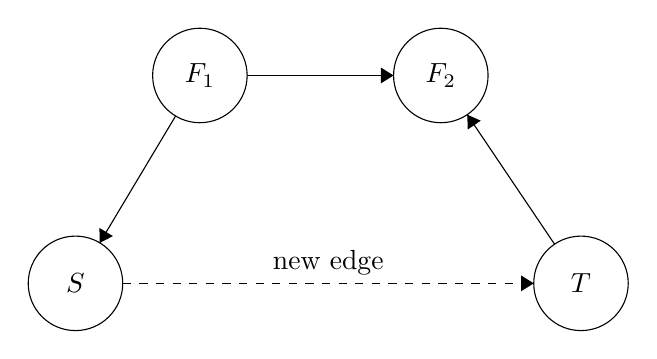
\begin{tikzpicture}[scale=0.2]
\tikzstyle{every node}+=[inner sep=0pt]
\draw [black] (18.1,-36.1) circle (3);
\draw (18.1,-36.1) node {$S$};
\draw [black] (50.2,-36.1) circle (3);
\draw (50.2,-36.1) node {$T$};
\draw [black] (26,-22.9) circle (3);
\draw (26,-22.9) node {$F_1$};
\draw [black] (41.3,-22.9) circle (3);
\draw (41.3,-22.9) node {$F_2$};
\draw [dashed] (21.1,-36.1) -- (47.2,-36.1);
\fill [black] (47.2,-36.1) -- (46.4,-35.6) -- (46.4,-36.6);
\draw (34.15,-35.6) node [above] {new edge};
\draw [black] (24.46,-25.47) -- (19.64,-33.53);
\fill [black] (19.64,-33.53) -- (20.48,-33.1) -- (19.62,-32.58);
\draw [black] (29,-22.9) -- (38.3,-22.9);
\fill [black] (38.3,-22.9) -- (37.5,-22.4) -- (37.5,-23.4);
\draw [black] (48.52,-33.61) -- (42.98,-25.39);
\fill [black] (42.98,-25.39) -- (43.01,-26.33) -- (43.84,-25.77);
\end{tikzpicture}
\end{center}
\caption{Two flip tolerant path.}
\label{figure_two_flip}
\end{figure}

Here, (S, $F_1$, $F_2$, T) is a two flip tolerant path. ($F_1$, S, T, $F_2$) is a new path, created because of the addition of (S,T), that conflicts with ($F_1$, $F_2$).

The two flip tolerant path search returns the set of all paths between a given source and sink that have up to two flips (paths that omit one or more of the three phases are also accepted).

The \textit{path extraction algorithm} then transforms the output of the two flip path search to the set of new pairs of parallel paths that arise in the diagram due to its addition, that need to be verified.

\paragraph{Path extraction algorithm}
The purpose of this algorithm is to derive the conflicting pairs that a given two-flip tolerant path corresponds to.

Let the new edge added to the diagram be (S, T).
It has already been shown how each path corresponds to a conflicting pair in the case where a path has two flips. When a path has only the first flip (which is to say, the third phase of the path is missing), but not the second flip, sink node T can be treated as the sink of the two conflicting path, while the first flipping point remains the source. Similarly when only the second flipping point is present then it is the sink, and S is the source. Finally when no flipping points are present, there are two possibilities. 
Either the path is oriented from S to T, in which case the conflicting paths are simply the edge (S, T) and the entire flip-less path, or the path is oriented from T to S. In this case, we have found a cycle, which has already been handled.

\paragraph{Theorem} Consider the result of two-flip tolerant path search from the source to sink node of an edge that is to be newly added followed with the path extraction algorithm described.  This result has a one-to-one correspondence to the set of new parallel pairs with exactly one path passing through the new edge and neither paths containing any cycles.

\paragraph{Proof}

Every element in the output of the path extraction algorithm was by construction a conflicting pair.

It remains to show that every new conflicting pair corresponds to a two flip tolerant path. Let the common source be $F_1$ and common sink be $F_2$. 

Only one path passes through (S, T), which we will name path 1. We construct a two flip tolerant path from S to T: phase 1 is the segment of path 1 from $F_1$ to S, phase 2 is path 2, and phase 3 is the segment of path 1 from T to $F_2$. It is possible that some of $F_1, F_2, S$ and $T$ coincide, in which case the corresponding segments between them disappear, and the resultant path has fewer than two flips.

We have shown that all paths that need verification are caught by the two flip tolerant search followed with path extraction.

\paragraph{Analysis}
This algorithm is also in the worst case as bad as factorial in the number of nodes. However, in the average case, it significantly outperforms the naive batch baseline. For sparse diagrams it is even competitive with our ultimate polynomial solution. Average case heuristic analysis will be presented in the evaluation section.

\subsection{Optimal batch solution}
Murota's main result ~\cite{commutative} is a solution to a batch version of \textsc{verification set} - given an acyclic diagram, it returns the minimal set of equality checks that would succeed if and only if the diagram commutes.
The paper describes the following algorithm to find the ($V^2E$ bounded) minimal set of pairs that needs to be checked.

A diagram's structure can result in some redundancy, in the sense that verifying a subset of pairs can imply the verification of path pairs that aren't in the subset.
For example, in figure ~\ref{figure_redundancies}, verifying $p_1$ and $p_2$ implies that the paths in $p_3$ are equal too.

\begin{figure}
    
\begin{center}
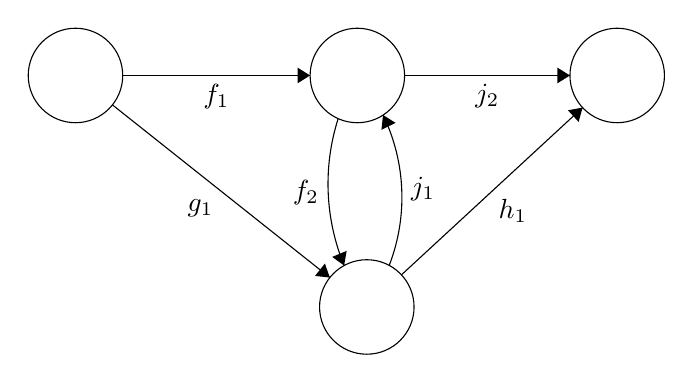
\begin{tikzpicture}[scale=0.2]
\tikzstyle{every node}+=[inner sep=0pt]
\draw [black] (12,-15.8) circle (3);
\draw [black] (30.5,-30.5) circle (3);
\draw [black] (46.4,-15.8) circle (3);
\draw [black] (29.9,-15.8) circle (3);
\draw [black] (15,-15.8) -- (26.9,-15.8);
\fill [black] (26.9,-15.8) -- (26.1,-15.3) -- (26.1,-16.3);
\draw (20.95,-16.3) node [below] {$f_1$};
\draw [black] (14.35,-17.67) -- (28.15,-28.63);
\fill [black] (28.15,-28.63) -- (27.84,-27.74) -- (27.21,-28.53);
\draw (19.94,-23.64) node [below] {$g_1$};
\draw [black] (29.063,-27.873) arc (-157.62406:-197.70132:13.638);
\fill [black] (29.06,-27.87) -- (29.22,-26.94) -- (28.3,-27.32);
\draw (27.49,-23.25) node [left] {$f_2$};
\draw [black] (31.53,-18.309) arc (25.84176:-21.16715:11.992);
\fill [black] (31.53,-18.31) -- (31.43,-19.25) -- (32.33,-18.81);
\draw (33.28,-23.03) node [right] {$j_1$};
\draw [black] (32.9,-15.8) -- (43.4,-15.8);
\fill [black] (43.4,-15.8) -- (42.6,-15.3) -- (42.6,-16.3);
\draw (38.15,-16.3) node [below] {$j_2$};
\draw [black] (32.7,-28.46) -- (44.2,-17.84);
\fill [black] (44.2,-17.84) -- (43.27,-18.01) -- (43.95,-18.75);
\draw (39.77,-23.64) node [below] {$h_1$};
\end{tikzpicture}

$p_1$=($f_1;f_2$, $g_1$)\\
$p_2$=($j_1;j_2$, $h_1$)\\
$p_3$=($f_1;h_1$, $f_1;j_2$)
\end{center}
\caption{Path checking redundancies: verifying $p_1$ and $p_2$ implies that the paths in $p_3$ are equal.}
\label{figure_redundancies}
\end{figure}

The approach in this algorithm, at a high level, is to define a function that takes in a subset of pairs and returns the subset of pairs whose verification is implied by verifying the input set. Then, greedy elimination of redundancies is performed until a minimal set is reached.

A bilinking is defined to be a parallel pair that is disjoint but for their terminal nodes. The set of all bilinkings is $R_0$.
In an acyclic diagram, if all bilinkings are equal, all parallel pairs must also be equal since they any given pair can be expressed as a composition of bilinkings.

Define $r_1>r_2$ for bilinkings $r_1$ = $\{p_l,q_l\}$, $r_2$= $\{p_2, q_2)$ $\in$ $R_0$, if there exists a path p such that $\partial p=\partial r_1$ and p contains $p_2$.
Define $\langle\rangle$ as:
$\langle r \rangle = \{ s\in R_0| r>s\}$.

For bilinking $s$, let $F(s)$ be the vector in $\mathbb{F}2^{|E|}$ representing the edges present in s (the $n^{th}$ dimension of $F(s)$ is 1 if the corresponding edge is in $s$, and 0 otherwise).
Let this function be extended to sets, so that for some set of bilinkings $S, F(S) = \{ F(s) | s\in S \}$. A notion of linear independence in this vector field exists.

For a set of bilinkings $r$, the closure function $cl$ is defined as:
\xxx[dg]{I think this definition is incomplete}\xxx[ak]{sorry, what is it missing?}
$cl(r) = \{ s\in R_0| s$ is linearly dependent on $F(r) \}$.

The closure function on $r$ basically captures all the pairs that can be made by made by composing or "gluing together" the bilinkings in r. 

Using these two function we finally define the function $\sigma$ on a set of bilinkings r as
$\sigma(r) = \{s \in R_0 | s\in cl(R\cap \langle s \rangle) \}$.
This is the function used to capture all the pairs whose verification is implied by the verification of pairs in r.

$\sigma$ is used to iteratively check if a given pair is redundant. Bilinkings are eliminated until a minimum "spanning" subset is reached.

% A complete implementation of the described algorithm is included in the appendix.

Roughly, it proceeds by first efficiently finding a "spanning" set of bilinkings (a subset whose verification implies the verification of all bilinkings in the graph).
It does this by, starting at every node, finding the reachable subsection of the graph, and a spanning tree for the subsection.
From each edges in the reachable section that is not a part of the tree, it generates a bilinking using the edge and a path in the tree that is parallel to the edge (algorithm ~\ref{algo_spanning_set}).

\xxx[dg]{Probably put this in the appendix}
\begin{algorithm}
\label{alg_spanning_set}
\DontPrintSemicolon
\KwResult{Find a spanning set Rs = [$r_1$, ... ,$r_k$].}

Graph existingGraph\;
$R_s$ $\gets$ \{\}\;
\ForEach{node v in V}{
    S $\gets$ existingGraph.extractReachableSection(v)\;
    T $\gets$ createMinimumSpanningTree(S)\;
    excludedEdges = S.edges - T.edges\;
    \ForEach{edge e $\in$ excludedEdges}{
        firstPath = T.findPath(source: e.source, sink: e.sink)\;
        $R_s$.addElement(new Bilinking(firstPath, e)\;
    } 
}
\KwRet{$R_s$}\;

\caption{finding spanning set}\label{algo_spanning_set}
\end{algorithm}

With the spanning set thus initialized, it greedily tries to remove each pair from the spanning set if the set remains spanning even after removing the edge (algorithm ~\ref{algo_minimal_spanning_set}).

\begin{algorithm}
\DontPrintSemicolon
\KwResult{Find a minimal spanning set R.}

\SetKwFunction{FSigma}{$\sigma$}
\SetKwProg{Fn}{Function}{:}{}
\Fn{\FSigma{inputSet S, codomain = Rs}}{
    output $\gets$ \{\}\;
    \For{bilinking $\in$ S}{
        smallerPairs $\gets$ \{\}\;
        \For{candidateBilinking $\in$ Rs}{
            \If{$\exists$ path from bilinking.source to candidateBilinking.source
            and
            $\exists$ path from candidateBilinking.sink to bilinking.sink}{
                \tcc{Check if there's a linear dependence between the bilinking and smallerPairs.
                    Vectorize(pair) returns a vector with a dimension for each edge in the graph,
                    with a 1 if pair includes that edge and 0 if it doesn't.}    
                matrix $\gets$ [vectorize(pair) for pair in smallerPair]\;
                matrix $\gets$ matrix+[vectorize(bilinking)]\;
                \If{determinant(matrix)\%2==0}{
                    output.add(bilinking)
                }
            }
        }
    }
    \KwRet{output}
}

R $\gets$ Rs\;
\For{i=1 to K}{
    \If{$r_i \in \sigma$(R-$r_i$)}{
       R $\gets$ R-$r_i$\;
    }
}
\KwRet{R}\;

\caption{Minimal spanning set}\label{algo_minimal_spanning_set}
\end{algorithm}

The proof of correctness can be found in Murota\cite{commutative}, 
The number of checks returned by the algorithm is at worst $O(|V|^2|E|)$. The overall run time of an optimized implementation is $O(|V|^4|E|^2)$.

\section{Solving the online addition problem}

We present a polynomial time solution to the \textsc{verification set} problem.
Like with the baseline, we do not concern ourselves with parallel pairs where neither or both paths pass through the new edge.
The key observation that allows us to improve on the online baseline is that, for a given source and sink pair, only a single parallel pair needs to be verified. 
This is an implication of Theorem \ref{reductionRule}, expanded on later.
Theorem \ref{verifyingSet} shows that should our selected set of pairs along with cycles passing through the new edge be verified commutative, the entire diagram must commute. 
The approach is to identify a parallel pair with exactly one path through the edge for each (source, sink) pair (algorithm ~\ref{algo_online_polynomial}).

\begin{algorithm}
\DontPrintSemicolon
\KwData{existing graph, new edge.}
\KwResult{Set of parallel pairs to verify.}
\SetKwProg{try}{try}{:}{}
\SetKwProg{catch}{catch}{:}{end}
Graph existingGraph;
Edge newEdge;

parallelPairs $\gets$ \{\}\;
\For{S in existingGraph.Nodes}{
    \For{T in existingGraph}{
        \try{}{
            Path pathWithNewEdge $\gets$ FindPath(
                graph: existingGraph, 
                sourceNode: S,
                sinkNode: newEdge.Source()) +\;
            newEdge as Path +\;
            FindPath(
                graph: existingGraph, 
                sourceNode: newEdge.Sink(), 
                sinkNode: T)\;
            \If{S == T}{
                pathInOldGraph $\gets$ identity(S)\;
            }
            \Else(){
                Path pathInOldGraph $\gets$ FindPath(
                    graph: existingGraph, 
                    sourceNode: S, 
                    sinkNode: T)\;
            }
            parallelPairs.add((pathInOldGraph, pathWithNewEdge))\;
        }
        \catch{PathFindingFailedException}{
           \tcc{No comparable pairs from node S to node T that need to be checked}
           continue\;
        }
    }
}
\KwRet{parallelPairs}\;
\caption{Online polynomial time algorithm to find parallel pair set}
\label{algo_online_polynomial}
\end{algorithm}

The try block is executed at most $O(|V|^2)$ times, so that this is the bound on the number of pairs verified.

The bound is asymptotically tight. This can be seen in the case where the graph contains 2N nodes besides S and T. We consider N of the nodes to be in group 1, and the other N to be in group 2. Every node in group 1 has a forward node to every node in group 2, as well as to S. T has a forward edge to every node in group 2. In this diagram, on the addition of edge (S, T), $N^2$ paths need to be verified which is polynomial in 2N+2.

Also notice that if trying to optimize for path length (say, if composing functions is expensive) then "find any path" can be replaced with "find shortest path".

An efficient implementation of the algorithm can run in $O(|V|^2(|V|+|E|))$ time at a $O(|V|^3)$ space cost. In such an implementation, path finding from a given source node to all potential sink nodes could be done in a single $O(|V|+|E|)$ breadth first search and the results memoized in $O(|V|^2)$ space.

\subsection{Optimization Step}

In the case where equality checks are very expensive, we begin by finding the minimal set of (source, sink) pairs such that checking for these pairs logically implies having checked the full diagram.

We observe that there are some redundancies in the diagram.

Consider the situation in figure ~\ref{figure_reduction_rule}.

\begin{figure}
\begin{center}
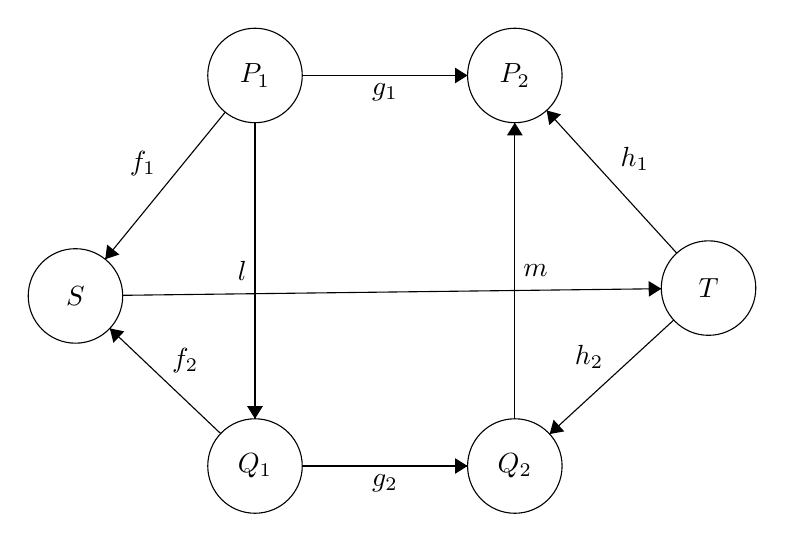
\begin{tikzpicture}[scale=0.2]
\tikzstyle{every node}+=[inner sep=0pt]
\draw [black] (16.6,-34.1) circle (3);
\draw (16.6,-34.1) node {$S$};
\draw [black] (56.8,-33.6) circle (3);
\draw (56.8,-33.6) node {$T$};
\draw [black] (28,-20.1) circle (3);
\draw (28,-20.1) node {$P_1$};
\draw [black] (44.5,-20.1) circle (3);
\draw (44.5,-20.1) node {$P_2$};
\draw [black] (28,-44.9) circle (3);
\draw (28,-44.9) node {$Q_1$};
\draw [black] (44.5,-44.9) circle (3);
\draw (44.5,-44.9) node {$Q_2$};
\draw [black] (31,-20.1) -- (41.5,-20.1);
\fill [black] (41.5,-20.1) -- (40.7,-19.6) -- (40.7,-20.6);
\draw (36.25,-20.6) node [below] {$g_1$};
\draw [black] (26.11,-22.43) -- (18.49,-31.77);
\fill [black] (18.49,-31.77) -- (19.39,-31.47) -- (18.61,-30.84);
\draw (21.74,-25.67) node [left] {$f_1$};
\draw [black] (25.82,-42.84) -- (18.78,-36.16);
\fill [black] (18.78,-36.16) -- (19.01,-37.08) -- (19.7,-36.35);
\draw (23.57,-39.02) node [above] {$f_2$};
\draw [black] (31,-44.9) -- (41.5,-44.9);
\fill [black] (41.5,-44.9) -- (40.7,-44.4) -- (40.7,-45.4);
\draw (36.25,-45.4) node [below] {$g_2$};
\draw [black] (54.59,-35.63) -- (46.71,-42.87);
\fill [black] (46.71,-42.87) -- (47.64,-42.7) -- (46.96,-41.96);
\draw (49.21,-38.76) node [above] {$h_2$};
\draw [black] (54.78,-31.38) -- (46.52,-22.32);
\fill [black] (46.52,-22.32) -- (46.69,-23.25) -- (47.43,-22.57);
\draw (51.19,-25.39) node [right] {$h_1$};
\draw [black] (28,-23.1) -- (28,-41.9);
\fill [black] (28,-41.9) -- (28.5,-41.1) -- (27.5,-41.1);
\draw (27.5,-32.5) node [left] {$l$};
\draw [black] (19.6,-34.06) -- (53.8,-33.64);
\fill [black] (53.8,-33.64) -- (52.99,-33.15) -- (53.01,-34.15);
\draw [black] (44.5,-41.9) -- (44.5,-23.1);
\fill [black] (44.5,-23.1) -- (44,-23.9) -- (45,-23.9);
\draw (45,-32.5) node [right] {$m$};
\end{tikzpicture}
Each arrow represents a path, and (S,T) is the new edge being added.
\end{center}
\caption{Reduction rule.}
\label{figure_reduction_rule}
\end{figure}

\begin{theorem}
\label{reductionRule}
If conflicting paths $g_2 = f_2; (S,T); h_2$ then it must be that $g_1 = f_1; (S,T); h_1$.
\end{theorem} 
% monomorphisms
\begin{proof}
We use the fact that $f_1$=$l; f_2$ and $h_1$=$h_2; m$.
\[g_2 = f_2; (S,T); h_2 \Rightarrow l; g_2 = l; f_2; (S,T) ; h_2 \]
\[\Rightarrow l ; g_2 ; m = l ; f_2 ; (S,T) ; h_2 ; m \Rightarrow g_1 = f_1 ; (S,T) ; h_1\]
\end{proof}

The proof is not affected if any of these paths is the identity, eg. if $f_1$ is the identity and S and $P_1$ are actually the same node.

We conclude that verifying a comparable pair of paths with end points ($P_1$, $P_2$) implies the verification of all path pairs ($Q_1$, $Q_2$) such that $Q_1$ is a successor of $P_1$ and $P_2$ is a successor of $Q_2$. A successor S to node N is any node such that there exists a path from N to S. Nodes are also their own successors and predecessors.

Under the assumption that the only path operations allowed are composition and replacement of one path by a different, equal path, as would be true when edges are generic functions, and no other information is available, so that F is a semi-group, this "reduction" rule is also the only rule to reduce the set of path pairs to check by finding implications.

That is to say, if verifying a comparable pair of paths with end points ($P_1$, $P_2$) implies the verification of a pair with endpoints ($Q_1$, $Q_2$), then it must be that $Q_1$ is a successor of $P_1$ and $P_2$ is a successor of $Q_2$. %TODO proof required?

Using this information it is possible to choose a minimal subset of path pairs to verify, as in algorithm ~\ref{algo_online_minimal}.

We construct a graph with a node for each possible (source, sink) pair in the graph- each node then represents a possible choice for parallel pair endpoint pairs, and greedily search for the smallest set of nodes from which the entire graph would be reachable. The idea is to look for "roots" in the graph that have to be included in the ultimate verification set because they have no predecessor an cannot be verified "through" the verification of some other pair. Then all the successors whose verification is implied by the roots are eliminated.

\begin{algorithm}
\DontPrintSemicolon
\KwData{Existing graph, new edge.}
\KwResult{Set of parallel pairs to verify.}
Graph existingGraph\;
Edge (S, T)\;
        
predecessors $\gets$ S.predecessors(existingGraph)\;
successors $\gets$ T.successors(existingGraph)\;

Graph terminalPairGraph\;
\For{q $\in$ successors}{
    \For{p $\in$ predecessors}{
        terminalPairGraph.addNode(q, p)\;
        \For{qPred $\in$ q.predecessors(existingGraph)}{
            \For{pSucc $\in$ p.successors(existingGraph)}{
                terminalPairGraph.addEdge((qPred, pSucc))\;
            }
        }
    }
}

verificationSet $\gets$ \{\}\;
\While{len(terminalPairGraph.nodes) $>$ 0}{
    currentNode $\gets$ terminalPairGraph.nodes[0]\;
    visitedNodes $\gets$ \{\}\;
    \While{len(currentNode.parents()) $>$ 0}{
        visitedNodes.add(currentNode)\;
        currentNode $\gets$ currentNode.parents()[0]\;
        \If{currentNode $\in$ visitedNodes}{
            edges $\gets$ getAllEdges(visitedNodes, terminalPairGraph)\;
            terminalPairGraph.removeNodes(visitedNodes)\;
            terminalPairGraph.addNode(currentNode, edges)\; 
        }
    }
    verificationSet.add(currentNode)\;
    terminalPairGraph.removeNodes( currentNode.successors(terminalPairGraph))\;
}
\KwRet{verificationSet}\;
\caption{Minimal set finding algorithm}
\label{algo_online_minimal}
\end{algorithm}

The result of the algorithm cannot be further reduced.
Also, the verification of the parallel pairs returned in the algorithm implies that the output of the previous algorithm must commute, and transitively with Theorem ~\ref{verifyingSet} that the entire diagram must commute.

The run time of the first step is $O(|V|^4)$, and that of the second step is $O(|V|)$, so that the overall bound is $O(|V|^4)$.

\subsection{Verification}
Ultimately verification is performed by calling an equality oracle (that is beyond the scope of this work) for every comparable pair returned by the previous stage, as in algorithm ~\ref{algo_verification}.

\begin{algorithm}
\DontPrintSemicolon
\For{(path1, path2) $\in$ parallelPairs}{
    \If{path1 $!$= path2}{
        \KwRet{False}\;
    }
}
\KwRet{True}\;
\caption{Verification algorithm}\label{algo_verification}
\end{algorithm}

\section{Applications}
TODO.

\subsection{Gator}

\subsection{Currency Graph}

To demonstrate our algorithms applied to a real world situation, 
we found inconsistencies in a diagram of the exchange rate between currencies.
Consider a diagram with nodes as currencies and a directed edge being the
conversion rate from its source node's currency to its sink node's currency.
Since the transformation exchange rate of money from any given base currency to a target currency
can be expected to be the same regardless of which intermediate currency transformations
are used, this diagram should commute.

Using an API ~\footnote{https://exchangeratesapi.io}, we built the fully connected diagram of exchange rates between 32 currencies on a given day.
To ensure that it indeed commuted, we started with an empty diagram, and added in edges one by one.
Before the addition of each edge, we used the algorithms (~\ref{algo_online_polynomial} and ~\ref{algo_online_minimal}) to ensure the addition of a new edge did not introduce inconsistencies in the existing diagram.
If a new edge was, in fact, problematic, the algorithms returned an example inconsistent
pair that would arise from the addition of the edge.
The pair would consist of two currency transformation sequences with the 
same source currency and ultimate destination currency, but with different effective 
exchange rates values, as computed by taking the product of all the exchange rates
encountered through the chain.

We allowed an "error tolerance", so that differences reported would not be the trivial consequences of a floating point error.
However, this relaxation of the equality oracle into imprecision meant that the mathematical reasoning that allow the algorithms to remove redundant path checks no longer applied.
For instance, composing a new function with two approximately equal functions does not lead to equal results, so theorem ~\ref{reductionRule} fails with this approximate equality.
When the algorithms reported no inconsistencies, it was still possible that the graph possessed inconsistencies above the given threshold and did not commute.
Nonetheless, both algorithms were effective in catching inconsistencies. Algorithm ~\ref{algo_online_polynomial} started finding inconsistencies at error tolerances to the order of $10^{-3}$, and ~\ref{algo_online_minimal}, which makes more invalid redundant path check removals, at error tolerances to the order of $10^{-7}$.

Averaging over evaluation for the first 30 days of 2020, building and verifying a diagram to completion (inclusive of the time required by network calls) took 243$\pm$19 seconds using algorithm ~\ref{algo_online_minimal}, and in 133$\pm$13 seconds with algorithm ~\ref{algo_online_polynomial}. 

\section{Evaluation}
We compare performance of the following path checking algorithms: (1) naive baseline (2) less naive, two-flip baseline (3) batch baseline (4) algorithm ~\ref{algo_online_polynomial}, and (5) algorithm ~\ref{algo_online_minimal}.
The two aspects we look at are time for response and size of response set (smaller sets -- tighter output results -- would mean less calls to the oracle).
We use randomly generated graphs for benchmarking, and vary their size.
Given a graph and a new edge, we time how long it takes for an algorithm to return  the set of pairs that need to be verified.
All computation was performed on a Macbook Pro 2015, 2.9 GHz Dual-Core Intel Core i5.

The naive baseline performs poorly, taking well over a thousand seconds for even small graphs of 10 nodes.
The batch algorithm brings timing down to seconds. Algorithm ~\ref{algo_online_polynomial} performs only slightly better.
Surprisingly, the optimal set algorithm cuts time cost by several orders of magnitude, and runs in milliseconds for small graphs.
All implementations are sensitive to density, performing better when density is very low or very high.

\subsection{Comparison of algorithm time cost}
The average time taken by each algorithm over the course of 10 runs over randomly generated graphs with 9 nodes and 32 edges is listed in table ~\ref{tab:times}.

\begin{table}
\begin{tabular}{|c|c|}
    \hline
    Algorithm & average seconds of computation \\
    \hline
    Naive baseline & 0.77 \\
    Two Flip tolerant & 0.075 \\
    Batch algorithm & 7.55 \\
    ~\ref{algo_online_polynomial} & 0.0038 \\
    ~\ref{algo_online_minimal} & 0.00086 \\
    \hline
\end{tabular}
\caption{Computation time for 9 node graph of density 0.4, averaged over ten runs}
\label{tab:times} %TODO debug and fix label not working.
\end{table}
    
\subsection{Scaling of time with input size}

Algorithms scale as expected with time, as seen in figure ~\ref{fig:timeVsSize}. 
Both ~\ref{algo_online_minimal} and ~\ref{algo_minimal_spanning_set} exhibit graphs that are polynomial in appearance, as does the batch baseline.
\xxx[AK]{Do I need to justify this by doing some kind of fit?}
The naive baseline as well as the two flip tolerant baseline display growth that quickly makes computation untenable.
The batch algorithm also grows fast, though not as much as the online checking baselines.

We define density to be the ratio of the number of edges in the graph to the total possible number of edges ($|V|^2$, where $|V|$ is the number of nodes).
Run time relates to the density of edges in the input graph.
The degree of the effect differs with the algorithms, as figure ~\ref{fig:timeVsSize} shows.
Generally, denser graphs entail longer computation time.
For the batch algorithm we use lower densities since the input graph must be acyclic. This puts an upper bound on density that approaches 0.5 in large graphs.
% Our proposed algorithms, ~\ref{algo_minimal_spanning_set} and ~\ref{algo_online_polynomial} are less affected because they aggressively remove redundancies.

\begin{figure}
    % TODO format nicely.
    \begin{subfigure}{.4\textwidth}
      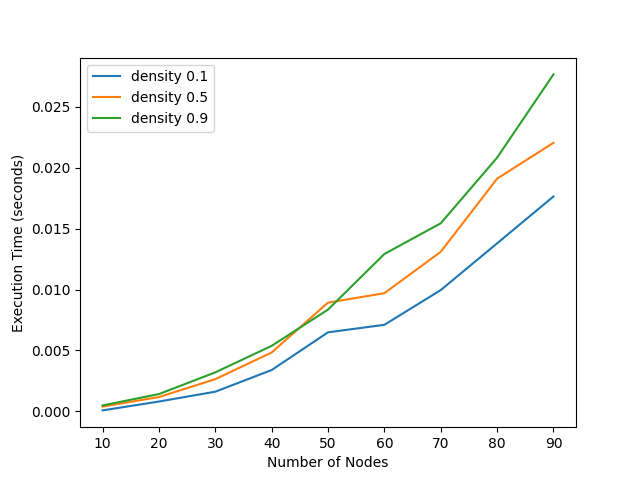
\includegraphics[width=.8\linewidth]{timeVsSize_10_OptimalSet.png}
      \caption{~\ref{algo_online_minimal}}
      \label{fig:sfigOptimalTvsS}
    \end{subfigure}

    \begin{subfigure}{.4\textwidth}
      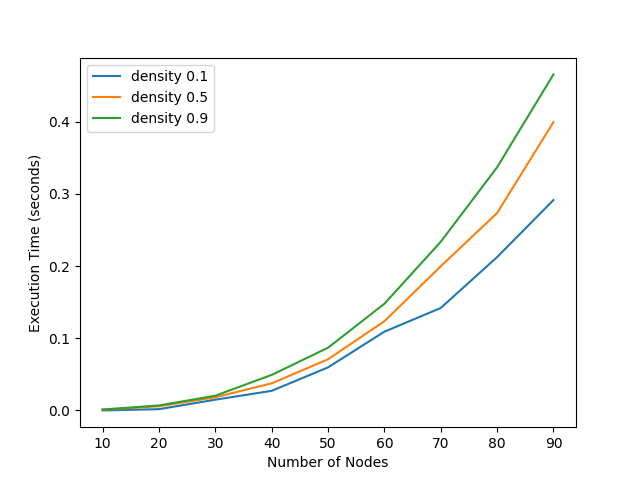
\includegraphics[width=.8\linewidth]{timeVsSize_10_Polynomial.png}
      \caption{~\ref{algo_online_polynomial}}
      \label{fig:sfigPolynomialTvsS}
    \end{subfigure}
    
    \begin{subfigure}{.4\textwidth}
      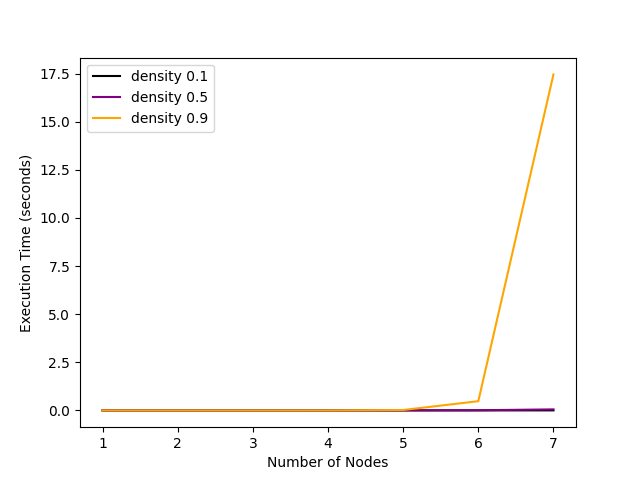
\includegraphics[width=.8\linewidth]{timeVsSize_10_NaiveChecker.png}
      \caption{Naive baseline}
      \label{fig:sfigNaiveTvsS}
    \end{subfigure}

    \begin{subfigure}{.4\textwidth}
      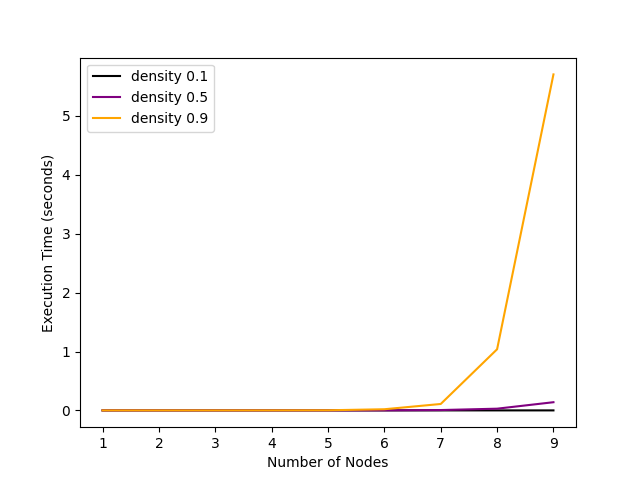
\includegraphics[width=.8\linewidth]{timeVsSize_10_TwoFlipPathChecker.png}
      \caption{Two flip tolerant baseline}
      \label{fig:sfigTwoFlipTvsS}
    \end{subfigure}

    \begin{subfigure}{.4\textwidth}
      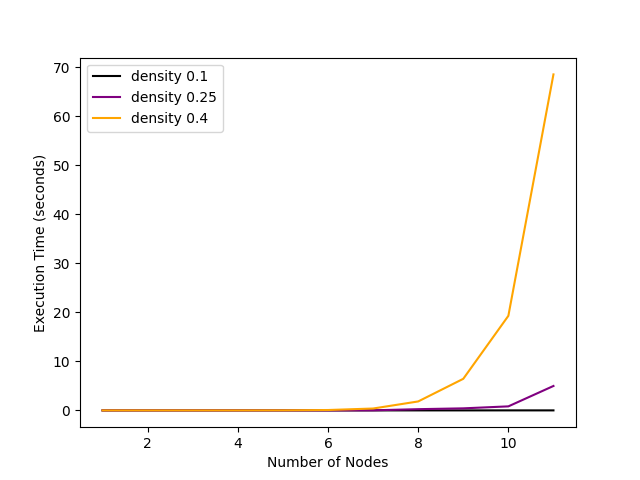
\includegraphics[width=.8\linewidth]{timeVsSize_10_BatchChecker.png}
      \caption{Batch algorithm baseline}
      \label{fig:sfigBatchTvsS}
    \end{subfigure}
    \caption{Plots of scaling of time with input size and density}
    \label{fig:timeVsSize}
\end{figure}

\subsection{Variance}
The periodic spikes in figure ~\ref{fig:sfigOptimalTvsS} are striking. 
We plot the spread of results to understand what is happening.
We find ~\ref{algo_online_minimal} has outliers about two standard deviation above the mean responsible for the spikes in the average.
The outliers themselves follow a polynomial curve.
The plots in figure ~\ref{fig:variance} depict the situation.
Grey points are the results of evaluation on individual points, and error bars show standard deviation. 
The black curve traces the mean.
No such effect is observed in ~\ref{algo_online_polynomial}.
\begin{figure}
    % TODO format nicely.
    \begin{subfigure}{.4\textwidth}
      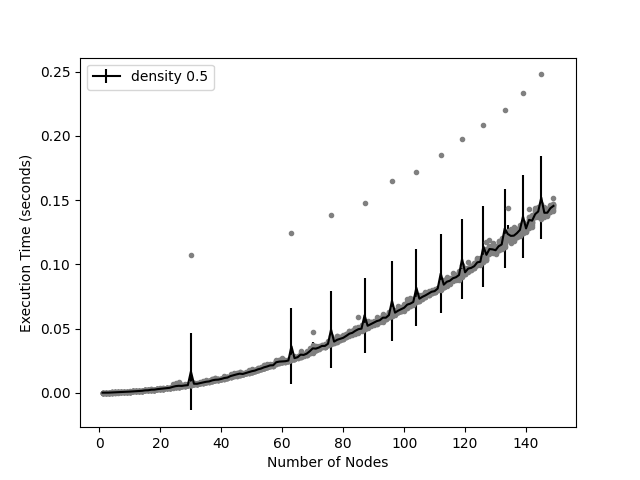
\includegraphics[width=.8\linewidth]{variance_10_OptimalSet.png}
      \caption{~\ref{algo_online_minimal}}
      \label{fig:sfigOptimalSpread}
    \end{subfigure}

    \begin{subfigure}{.4\textwidth}
      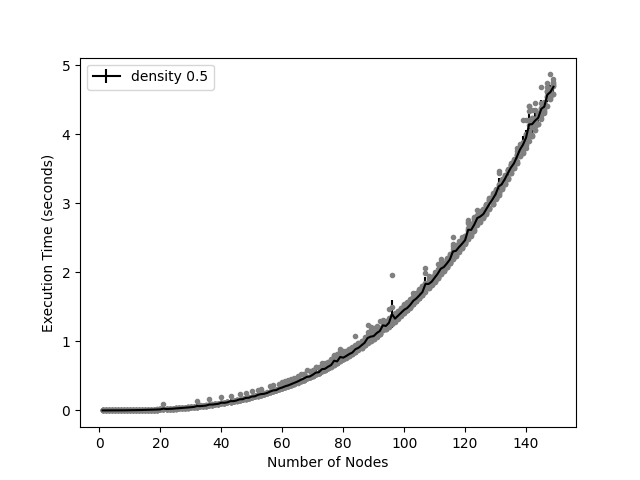
\includegraphics[width=.8\linewidth]{variance_10_Polynomial.png}
      \caption{~\ref{algo_online_polynomial}}
      \label{fig:sfigPolynomialSpread}
    \end{subfigure}
    
    \begin{subfigure}{.4\textwidth}
      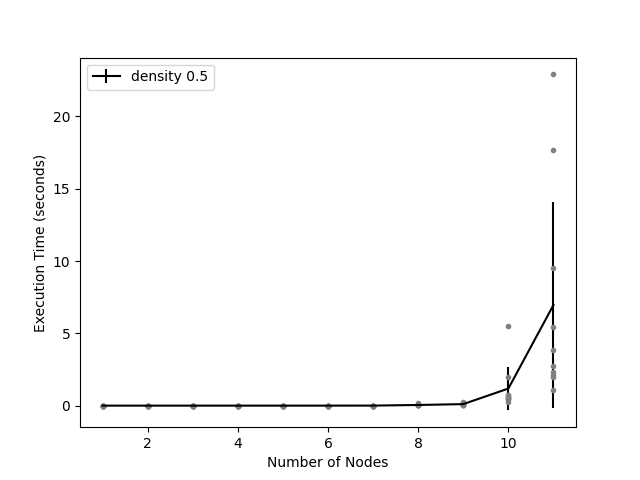
\includegraphics[width=.8\linewidth]{variance_10_TwoFlip.png}
      \caption{Two flip tolerant baseline}
      \label{fig:sfigTwoFlipSpread}
    \end{subfigure}

    \caption{Plots of spread of results}
    \label{fig:variance}
\end{figure}

\subsection{Size of Output}
Output size is a metric of interest, should the equality checking oracle be expensive.
Table ~\ref{tab:sizes}, summarizes the number of output pairs that the algorithms returned on average over 10 runs, for graphs with 9 nodes and 32 edges.
\begin{table}
\begin{tabular}{|c|c|}
    \hline
    Algorithm & average number of output pairs \\
    \hline
    Naive baseline & 39754.9 \\
    Two Flip tolerant & 748.9 \\
    Batch algorithm & 23 \\
    ~\ref{algo_online_polynomial} & 78.3 \\
    ~\ref{algo_online_minimal} & 1 \\
    \hline
\end{tabular}
\caption{Output size for 9 node graph of density 0.4, averaged over ten runs}
\label{tab:sizes}
\end{table}

\section{Appendix: Theorems and additional cases}

Consider all the cycles in the graph that pass through the new edge, unique to their terminal point.
Define a cycle-pair corresponding to cycle c to mean the pair of paths (c, identity on terminal node of c).
Let $C$ be the set of all cycle-pairs (unique to their terminal point) corresponding to cycles that pass through the new edge.

Let V, the set of pairs to verify, be $C \cup R_0$.

\begin{lemma}
\label{one_occurence_lemma}
A path that involves the new edge more than once is equal to a path without multiple occurrences of the edge, under the assumption that the pairs in C are verified.
\end{lemma}
\begin{proof}
Consider the part of the path between the first occurrence of the new edge and the second. This forms a cycle, which has a corresponding check in $C$ and must be verified to be equal to the identity.
This means that the loops containing the multiple occurrences of the new edge may be ignored and the path with a single occurrence of the new edge with the cycles removed is equal to this path.
\end{proof}

\begin{theorem}
\label{verifyingSet}
Verifying that all pairs in V commute implies that all pairs in $R_{all}$ commute.
\end{theorem}
\begin{proof}

Each pair in $R_{all}$ that is not in V would fall into one of these categories:

Case A: pairs that do not involve the new edge: By assumption that the original diagram commutes, these pairs must commute.

Case B: Cases where there is a different pair corresponding to this choice of (source, sink) in V already.
There are four paths to be considered, two from each pair. Those paths which do not include the new edge must already be equal by the assumption that the original diagram commutes.
Those paths which do include the new edge (S,T) can be reduced, by the case for multiple occurrences of a new edge, to a path with a single occurrence of the new edge as described in the preceding lemma \ref{one_occurence_lemma}. These new paths can be divided into three segments: the segment from the source to S, the new edge, and the segment from the last occurrence of T to the sink. The first segments of all paths are equal by assumption that the original diagram commutes. This is also true of the third segment of all the paths. The second segment consists of only the new edge and is the same for all paths. The composition of equal functions is equal, so all the paths passing through the new edge must be equal.
Therefore it is sufficient to check one path that passes through the new edge and one that doesn't. Such a pair belongs to V by construction.
\end{proof}

\section{Case Studies}

\bibliography{refs}
\bibliographystyle{plain}

\end{document}
